\begin{figure}[!ht]
  \centering
  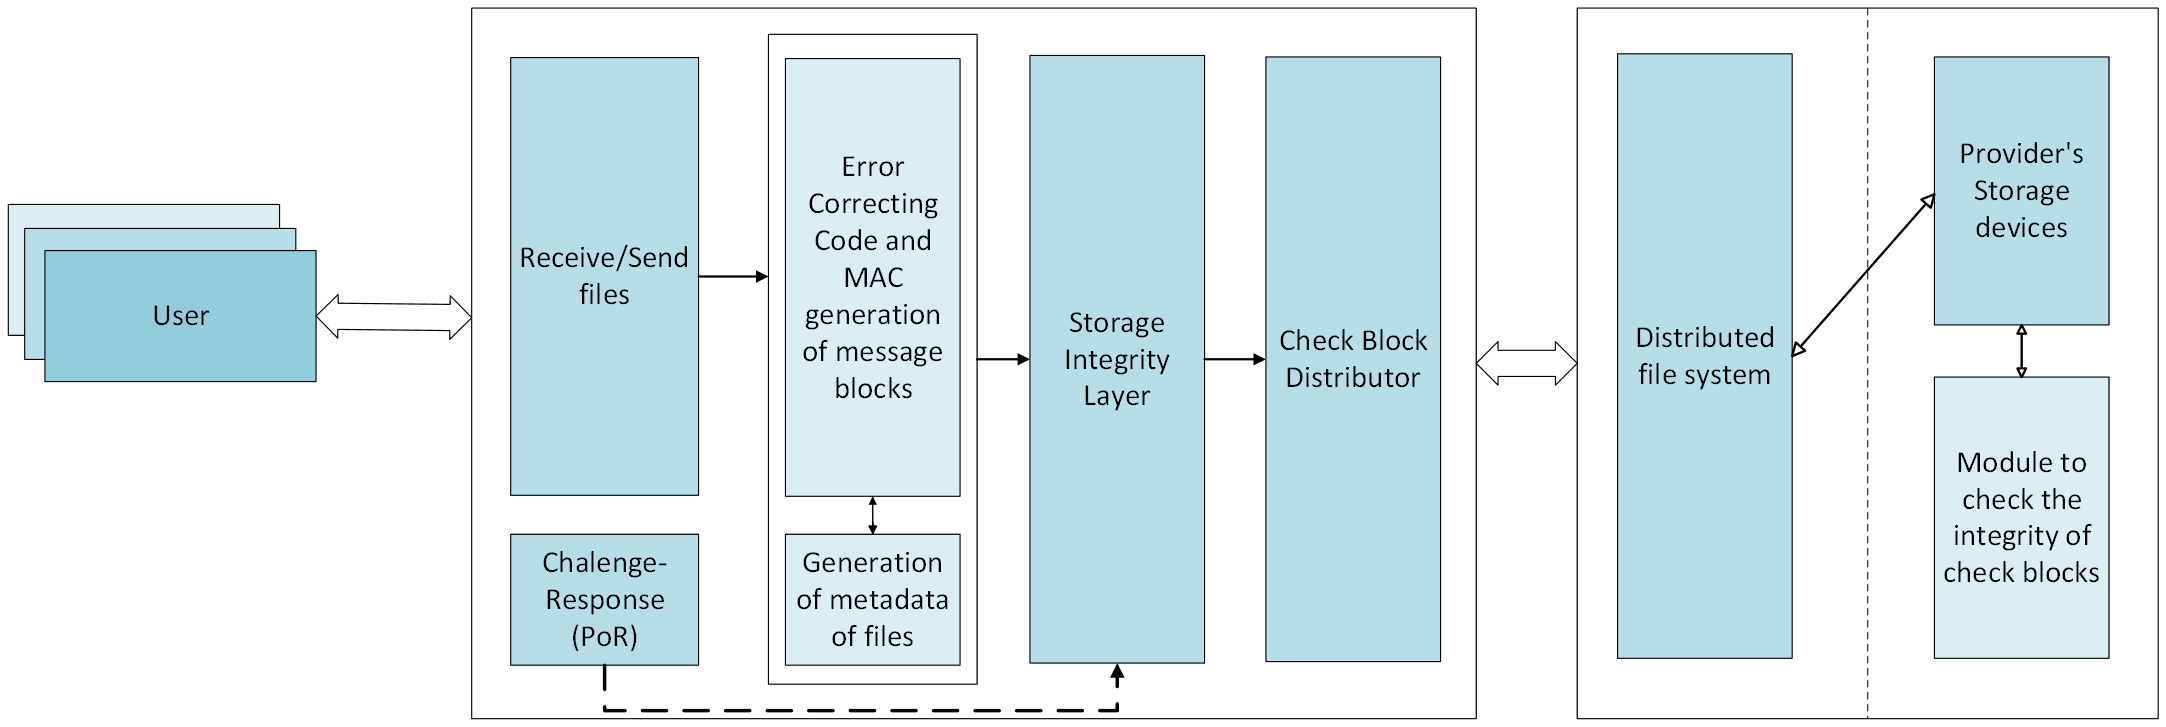
\includegraphics[width=\textwidth]{img/Hysail-Architecture.png}
  \caption{Visão geral das fases centrais do HySail.}
\end{figure}

HySail combina três ideias que aparecem de forma explícita: códigos corretivos do tipo 
\emph{Online Codes} para ampliar disponibilidade, uma representação polinomial sobre corpos de Galois para
verificar integridade e um protocolo de auditoria do tipo \emph{proof of retrievability} para ligar ambas as
propriedades ao armazenamento em nuvem. Na prática, o arquivo \(F\) é dividido em blocos, redundâncias são
geradas por XOR e os blocos resultantes são distribuídos entre provedores distintos. Em paralelo, o cliente
guarda autenticações algébricas suficientes para verificar se os blocos reconstruídos continuam coerentes com
o estado original do arquivo.

\section{Online Codes (Fountain Codes)}%
Um dos pontos necessários para garantir que a disponibilidade do HySail seja alta é o uso de \emph{erasure codes} do tipo \emph{Online Codes},
uma classe de \emph{Fountain Codes} rateless: o codificador pode continuar produzindo símbolos redundantes até que a quantidade de informação
recuperável seja suficiente para reconstruir \(F\)~\cite{amaral2013hysail}.

Se o arquivo original é particionado em \(n\) blocos
\[
F = \{m_i\}_{i=1}^{n},
\]
o processo de codificação gera um arquivo composto \(F' = \{m'_i\}_{i=1}^{n'}\) com
\[
n' = (1 + k\delta)n,
\]
em que \(\delta\) é a taxa de redundância excedente do código. Os \(n k \delta\) blocos adicionados nessa etapa são
chamados de blocos auxiliares e são obtidos como XOR de subconjuntos dos blocos originais. Em seguida, o
codificador produz os blocos de verificação \(c_i\), que também são XOR de um subconjunto dos blocos do arquivo
composto.

Essa estrutura é importante porque o HySail não depende de um provedor específico. Os blocos podem ser
distribuídos entre \(N\) provedores \(S = \{S_1, \ldots, S_N\}\), e a reconstrução pode ser feita a partir de um
conjunto suficiente de blocos não corrompidos. O resultado prático é que a disponibilidade não vem da
duplicação simples, mas da combinação entre redundância algébrica e distribuição em múltiplos provedores.

O próprio processo de decodificação reforça essa ideia: blocos de grau 1 são recuperados primeiro, pois são
cópias diretas de um bloco original. A partir deles, blocos de grau maior podem ser resolvidos iterativamente
por XOR até que todos os blocos do arquivo original sejam obtidos.

\section{Representação no corpo de Galois}%
No HySail, cada bloco de mensagem \(m_i\) é representado como um polinômio sobre \(GF(2^k)\). Em vez de
tratar o conteúdo apenas como bytes, o protocolo converte o bloco em coeficientes binários que é descrito por:
\[
m_i(x) = \sum_{r=0}^{t-1} a_r x^r, \qquad a_r \in \{0,1\}.
\]
Essa representação é utilizada no cálculo do autenticador homomórfico.

Através desta representação é possível garantir que em \(GF(2)\), soma e XOR são a mesma operação. Assim, se dois blocos são
combinados por XOR, a representação polinomial preserva o mesmo comportamento algébrico.
Antes que o bloco \(m_i\) seja enviado, o cliente escolhe um polinômio primitivo \(P_j(x)\) e calcula o resto da divisão polinomial
de cada bloco por esse polinômio:
\[
h_{i,j}(x) = m_i(x) \bmod P_j(x).
\]

Sendo que cada \(i\) refere-se ao bloco e \(j\) ao polinômio primitivo escolhido, sendo que o número de polinômios primitivos é \(l\),
o cliente mantém essa família de MACs para cada bloco gerado através da divisão polinomial, o que permite verificar a integridade dos blocos durante a auditoria sem precisar
manter o arquivo inteiro na memória.

Essa construção tem duas consequências diretas:
\begin{enumerate}
  \item O conjunto de MACs é pequeno e controlado pelo grau de \(P_j(x)\)
  \item O cliente pode comparar respostas agregadas sem precisar manter o arquivo
inteiro. A segurança depende do resto da divisão polinomial e do uso de polinômios primitivos de
grau \(\lambda\), o que leva à interpretação do MAC como uma família de funções hash 2-universais.
\end{enumerate}

Em termos de colisão, o protocolo garante que a probabilidade de dois blocos distintos produzirem o mesmo valor de
MAC é de ordem \(2^{-\lambda}\). Isso permite tratar \(h_{i,j}\) como uma validação de integridade de baixo custo,
formalmente associada ao bloco original.

\section{Codificação e Upload}%
Nesta etapa, é feita distribuição dos blocos utilizando os dois mecanismos já definidos: a redundância utilizando \emph{Online Codes}
e a autenticação polinomial em \(GF(2^k)\). Em termos de artefatos, o cliente produz os blocos de verificação
\(\{c_i\}_{i=1}^{t}\), calcula a família \(\{h_{i,j}\}_{i=1,j=1}^{n,l}\) e registra os metadados de
composição de cada bloco.

Esses metadados são importantes para as fases seguintes, pois identificam como cada \(c_i\) foi construído a
partir de XOR de blocos-base. Por exemplo, se
\[
c_8 = m_1 \oplus m_5 \oplus m_{11} \oplus m_{128},
\]
o registro correspondente é \(\langle 8, \{1,5,11,128\} \rangle\). Com isso, o sistema preserva de forma
reduzida, a informação necessária tanto para reconstrução quanto para auditoria.

No upload, os blocos de verificação são distribuídos entre provedores \(S_i\), enquanto o cliente mantém os
MACs e os metadados locais. Essa separação de responsabilidades reduz o impacto de falhas isoladas e prepara o
ambiente para a decodificação e para os desafios de integridade apresentados nas seções seguintes.

\section{Reconstrução}%

A reconstrução no HySail combina decodificação iterativa e recomposição de redundância. O objetivo é recuperar
os \(n\) blocos originais a partir de um subconjunto íntegro de blocos codificados, desde que a quantidade
disponível atinja o limiar mínimo de recuperabilidade,
\[
\tau = (1-\delta)(1+k\delta)n.
\]

O processo inicia pela identificação de blocos de grau 1, que revelam diretamente um bloco de mensagem.
Em seguida, os blocos já recuperados são substituídos nas demais equações de XOR, reduzindo o grau dos blocos
restantes até que novos blocos de grau 1 apareçam. O ciclo se repete até a recuperação completa do arquivo.
Em notação simplificada, a reconstrução resolve sucessivamente relações do tipo
\[
c_i = \bigoplus_{r \in X_i} m_r,
\]
isolando o único \(m_r\) desconhecido quando os demais termos de \(X_i\) já são conhecidos.

Como exemplo, se
\[
c_{12} = m_1 \oplus m_7 \oplus m_9 \oplus m_{14}
\]
e \(m_7\), \(m_9\) e \(m_{14}\) já foram recuperados, então
\[
m_1 = c_{12} \oplus m_7 \oplus m_9 \oplus m_{14}.
\]

A redundância introduzida pelos \emph{Online Codes} não é apenas a base para recuperação do arquivo, mas também
do sistema de detecção e correção de erros.

\section{Correção de Erros}%
O mecanismo de correção de erros do HySail aproveita o fato de que blocos de verificação são construídos por XOR
de blocos iniciais. Quando a auditoria identifica um bloco corrompido, o cliente não precisa solicitar
ao provedor uma retransmissão: ele pode recompor o bloco perdido a partir de outros blocos de verificação cuja
integridade foi validada.

Formalmente, se um bloco \(c_j\) foi detectado como corrompido e o cliente possui blocos \(c_{j_1}, c_{j_2}, \ldots, c_{j_k}\)
integros cuja composição por XOR produz a informação necessária, o bloco pode ser recuperado por
\[
c_j = c_{j_1} \oplus c_{j_2} \oplus \cdots \oplus c_{j_k}.
\]
Esse processo é idêntico ao da decodificação, mas aplicado à camada de verificação em vez de à camada de mensagem.

Um aspecto crucial é que a correção não é imediata após um desafio, ela é acionada apenas quando a auditoria
detecta violação do limiar de integridade. O protocolo define que, detectada a corrupção, o cliente recompõe o bloco
inválido e o redistribui para outro provedor. Essa operação garante que a
malha de redundância seja restaurada, permitindo que futuras rodadas de auditoria continuem efetivas.

Essa etapa é uma redistribuição do código, não regenera o arquivo inteiro, apenas o bloco
que foi identificado como corrompido. Essa eficiência é possível pela separação de responsabilidades, o cliente mantém os
metadados de composição localmente e pode operar sobre blocos isolados sem precisar do contexto completo.

\section{Auditoria}%
HySail permite dois modelos de auditoria, \textit{bounded} e \textit{unbounded}. Em ambos, o cliente escolhe um polinômio
primitivo \(P_j(x)\) e verifica um subconjunto de blocos por meio de um desafio-resposta. No modelo \textit{bounded},
o cliente envia também os índices dos blocos que devem ser testados. Por exemplo, se o desafio é para os blocos \(m_1\), \(m_5\) e \(m_{11}\), o cliente espera receber
\[
A(x) = \left(\bigoplus_{\eta \in \mathrm{list}} c_\eta(x)\right) \bmod P_j(x).
\]

O ponto central é que a função MAC é homomórfica em relação a XOR. Se
\[
m_a(x) \bmod P_j(x) = \sigma_{a,j}(x) \quad \text{e} \quad m_b(x) \bmod P_j(x) = \sigma_{b,j}(x),
\]
então para o bloco composto \(c_e = m_a \oplus m_b\) vale
\[
\sigma_{a,j}(x) \oplus \sigma_{b,j}(x) = (m_a(x) \oplus m_b(x)) \bmod P_j(x).
\]
Em outras palavras, a verificação de um bloco agregado pode ser reduzida à combinação das autenticações
individuais. Isso explica por que HySail pode auditar blocos de verificação sem manter o arquivo completo na
memória do cliente.

O protocolo também formaliza o lado de segurança. A família de MACs é tratada como uma função hash
2-universal, com probabilidade de colisão da ordem de \(2^{-\lambda}\), onde \(\lambda\) é o grau do
polinômio primitivo. Para a recuperabilidade, a probabilidade de sucesso é dada por
\[
1 - \delta^k,
\]
de modo que a falha de recuperação permanece pequena quando \(\delta^k\) é negligenciável. Somando as duas
fontes de falha, a chance total de erro é:
\[
\Pr[\mathrm{Fail}] = 2^{-\lambda} + \delta^k,
\]
o que tende a zero conforme os parâmetros do esquema crescem.

\section{Modelo adversarial e segurança}%
O modelo adversarial do artigo considera um conjunto de provedores \(S = \{S_1, \ldots, S_N\}\), ligado a
uma entidade confiável \(T\), e admite corrupção por uma fração limitada de blocos. A ideia é que um atacante pode
alterar blocos, apagar conteúdos ou explorar falhas temporárias, mas ainda assim não consegue comprometer a
segurança global se a quantidade de corrupção respeitar o limiar imposto pelos parâmetros do código.

Essa modelagem leva a dois limiares relevantes \(\tau_{provider}\), associado ao quanto cada provedor pode
perder antes de ser considerado inseguro, e \(\tau_{global}\), associado ao conjunto inteiro de blocos
distribuídos. Quando a auditoria detecta violação, a fase de redistribuição recompõe blocos corrompidos a partir
dos blocos remanescentes, novamente por XOR, sem exigir o download do arquivo completo.

Em termos conceituais, esse é o ganho do HySail a disponibilidade vem do código corretor e integridade vem do
MAC homomórfico. O resultado é uma camada de armazenamento em nuvem que tenta equilibrar recuperação prática,
auditoria barata e verificação consistente.
